% !TEX root = ../Projektdokumentation.tex
\section{Implementierungsphase} 
\label{sec:Implementierungsphase}

Bevor mit der Implementierung begonnen wurde, wurde ein Iterationsplan erstellt. In diesem wurden die einzelnen Schritte und deren Reihenfolge festgelegt. In jeder Iteration wurde eine spezifische Funktionalität umgesetzt und am Ende der jeweiligen Iteration dem Team präsentiert. Dieses Vorgehen folgt den in Abschnitt 2.3 beschriebenen Prinzipien der agilen Softwareentwicklung. Der vollständige Iterationsplan befindet sich im \Anhang{app:Iterationsplan}.

\subsection{Implementierung der Gitlab Systemhook}
\label{sec:ImplementierungDatenstrukturen}

\begin{figure}[htb]
	\centering
	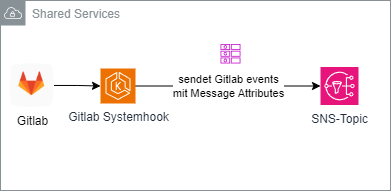
\includegraphics[scale=0.5]{systemhookOnly.drawio.png}
	\caption{Implementierung der Gitlab Systemhook}
\end{figure}

\subsection{Implementierung der GitLab Systemhook}
\label{sec:ImplementierungGitlabSystemhook}

Die Implementierung der GitLab Systemhook ermöglicht es, Ereignisse wie das Erstellen neuer Benutzer in GitLab zu erfassen und diese an ein SNS (Simple Notification Service) Topic weiterzuleiten. Der Service empfängt HTTP-POST-Anfragen von GitLab, validiert das Token und verarbeitet die Payload asynchron, um die Performance zu optimieren. 

Hierfür wurde das \texttt{Echo}-Framework in Kombination mit dem AWS SDK für Go eingesetzt. Zu Beginn wurde der Hook auf der Testumgebung des EKS-Clusters (Elastic Kubernetes Service) implementiert. Nach der erfolgreichen Validierung der Funktionalitäten wurde der Code schließlich in die Produktionsumgebung überführt. 

Ein Beispiel für die Handhabung der eingehenden Hooks ist in Listing~\ref{lst:handleHook} im Anhang zu finden, während die Logik zur Nachrichtenübermittlung an SNS in Listing~\ref{lst:publishMessage} dargestellt wird. Die Implementierung der Umgebungsvariablen und der Authentifizierung erfolgt im Codeabschnitt in Listing~\ref{lst:newHook}. 

Die gesamte Lösung ermöglicht eine effiziente und skalierbare Verarbeitung von GitLab-Ereignissen und deren gezielte Weiterleitung an AWS SNS, wodurch ein automatisierter Workflow für das Benutzer-Management geschaffen wird.

\subsection{Implementierung der Nachrichtenzustellung an SNS}
\label{sec:ImplementierungSNS}

Nach Empfang eines GitLab-Ereignisses wird die Nachricht, zusammen mit Attributen wie dem Eventnamen, an ein vordefiniertes SNS Topic gesendet. Ein Attributfilter stellt sicher, dass nur relevante Ereignisse wie \texttt{user\_create} verarbeitet werden. Dadurch wird eine gezielte Filterung und Weiterverarbeitung auf Empfängerseite ermöglicht.

\subsection{Bereitstellung und Test}
\label{sec:BereitstellungTest}

Der Service wurde zunächst auf einer Testumgebung des EKS-Clusters bereitgestellt. Nach erfolgreicher Validierung der Funktionalitäten erfolgte die Bereitstellung in der Produktionsumgebung. Die Lösung ermöglicht eine skalierbare Verarbeitung von GitLab-Ereignissen und deren Weiterleitung an AWS SNS.

2100 active user

150
150


\subsection{Implementierung des Dev-Kickstarter}
\label{sec:ImplementierungBenutzeroberflaeche}

\begin{itemize}
	\item Beschreibung der Implementierung der Benutzeroberfläche, falls dies separat zur Implementierung der Geschäftslogik erfolgt (\zB bei \acs{HTML}-Oberflächen und Stylesheets).
	\item \Ggfs Beschreibung des Corporate Designs und dessen Umsetzung in der Anwendung.
	\item Screenshots der Anwendung
\end{itemize}

\paragraph{Beispiel}
Screenshots der Anwendung in der Entwicklungsphase mit Dummy-Daten befinden sich im \Anhang{Screenshots}.


\subsection{Implementierung der E-Mail}
\label{sec:ImplementierungGeschaeftslogik}

\begin{itemize}
	\item Beschreibung des Vorgehens bei der Umsetzung/Programmierung der entworfenen Anwendung.
	\item \Ggfs interessante Funktionen/Algorithmen im Detail vorstellen, verwendete Entwurfsmuster zeigen.
	\item Quelltextbeispiele zeigen.
	\item Hinweis: Wie in Kapitel~\ref{sec:Einleitung}: \nameref{sec:Einleitung} zitiert, wird nicht ein lauffähiges Programm bewertet, sondern die Projektdurchführung. Dennoch würde ich immer Quelltextausschnitte zeigen, da sonst Zweifel an der tatsächlichen Leistung des Prüflings aufkommen können.
\end{itemize}

